\section{El Problema de la Mochila}
El problema de la mochila es un clásico en el ámbito de la optimización combinatoria y la teoría de algoritmos. Se trata de seleccionar un subconjunto de artículos, cada uno con un peso y un valor, de manera que se maximice el valor total sin exceder la capacidad de peso permitida. Este problema es fundamental en campos como la logística, la gestión de recursos y la toma de decisiones en la ingeniería. La programación dinámica y las técnicas de aproximación ofrecen métodos eficientes para resolver este problema.

\subsection{Ejemplo 1}
Un naviero tiene un buque carguero con capacidad de hasta 500 toneladas. El carguero transporta contenedores de diferentes pesos para una determinada ruta. En la ruta actual el carguero puede transportar algunos de los siguientes contenedores:

\begin{table}[H]
    \centering
    \begin{tabular}{cccccc}
        \toprule
        \textbf{Contenedor} & 1 & 2 & 3 & 4 & 5 \\
        \midrule
        Peso en (cientos de toneladas) & 1 & 2 & 1 & 3 & 4 \\
        Valor (miles de dólares) & 3 & 5 & 4 & 6 & 7 \\
        \bottomrule
    \end{tabular}
    \caption{Datos del problema de la mochila. Elaboración propia.}
    \label{tab:datos_contenedores}
\end{table}

El analista de la empresa del armador desea determinar el envío (conjunto de contenedores) que maximiza el valor de la carga transportada.

\subsubsection{Código}
\begin{lstlisting}[language=Python]
def algoritmo_mochila(pesos, valores, capacidad):
    n = len(pesos)
    matriz = []
    for i in range(n + 1):
        fila = []
        for j in range(capacidad + 1):
            fila.append(0)
        matriz.append(fila)

    for i in range(1, n + 1):
        for w in range(1, capacidad + 1):
            if pesos[i - 1] <= w:
                matriz[i][w] = max(matriz[i - 1][w], valores[i - 1] + matriz[i - 1][w - pesos[i - 1]])
            else:
                matriz[i][w] = matriz[i - 1][w]

    w = capacidad
    contenedores_seleccionados = []
    for i in range(n, 0, -1):
        if matriz[i][w] != matriz[i - 1][w]:
            contenedores_seleccionados.append(i)
            w -= pesos[i - 1]

    valor_maximo = matriz[n][capacidad]
    contenedores_seleccionados.reverse()
    return valor_maximo, contenedores_seleccionados
\end{lstlisting}

\subsubsection{Resultado}
\begin{figure}[H]
    \centering
    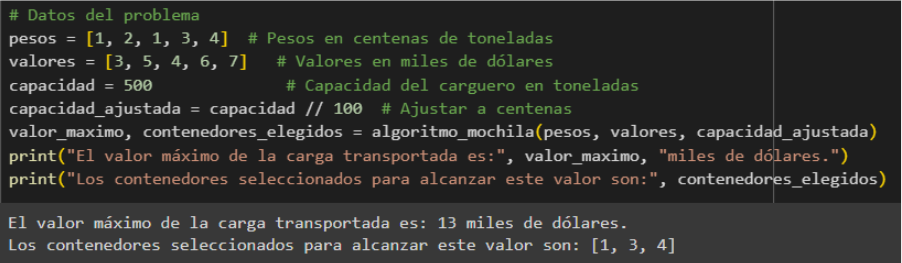
\includegraphics[width=0.8\textwidth]{resultado_mochila_ejem1.png}
    \caption{Imagen del resultado del código Python.}
    \label{fig:resultado_ejemplo1}
\end{figure}

\subsubsection{Análisis de complejidad}
\begin{figure}[H]
    \centering
    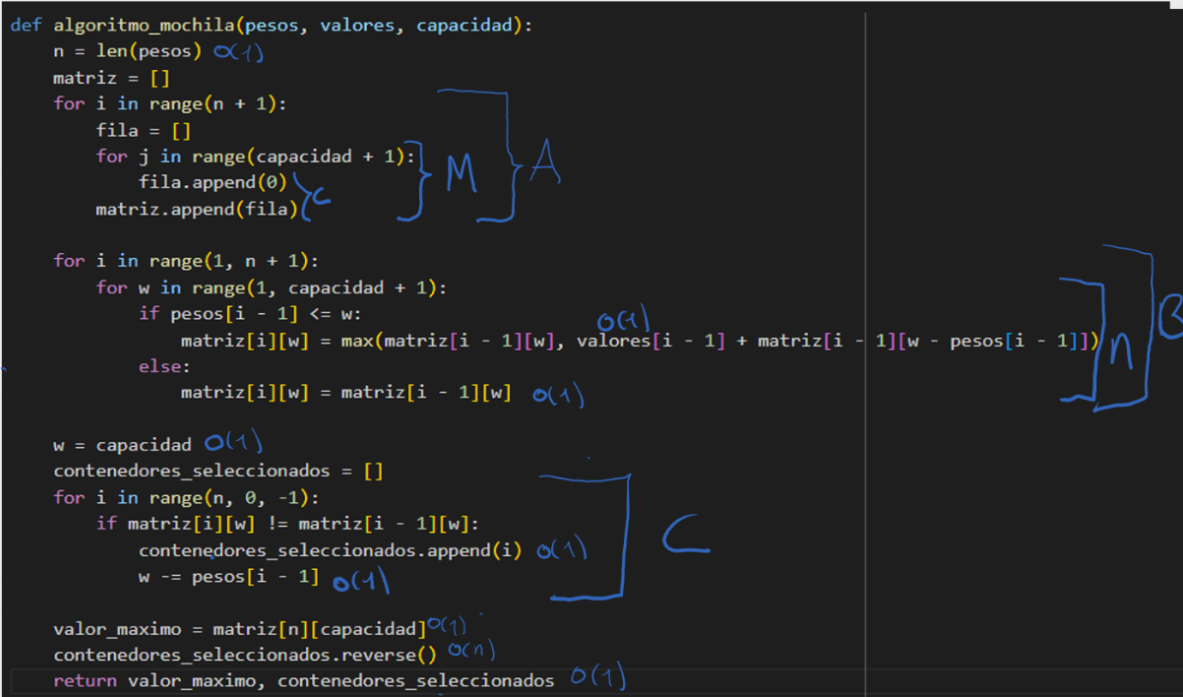
\includegraphics[width=0.8\textwidth]{complejidad_mochila_ejem1.png}
    \caption{Análisis del código.}
    \label{fig:complejidad_ejemplo1}
\end{figure}

\begin{figure}[H]
    \centering
    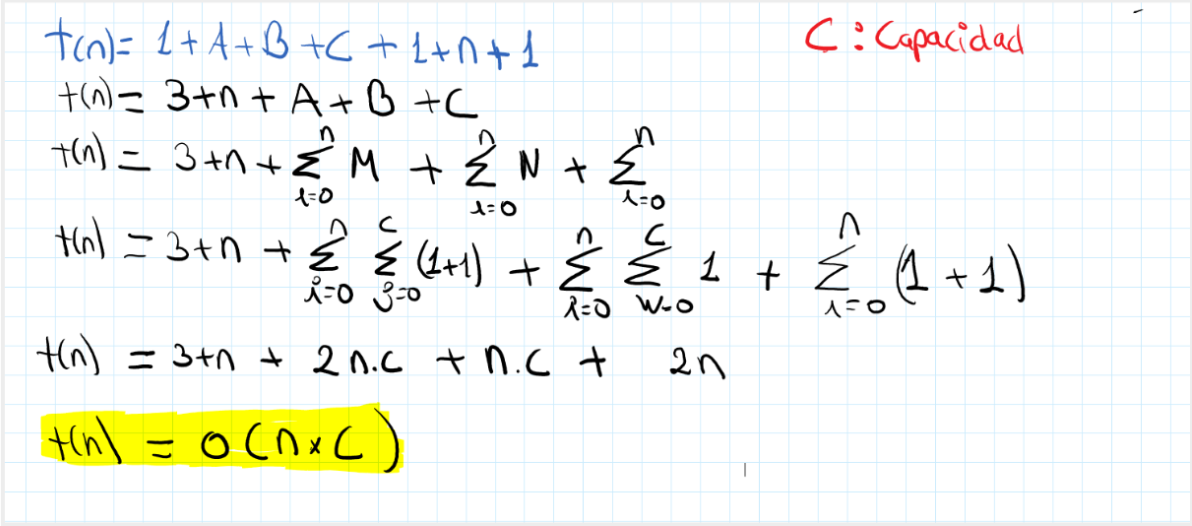
\includegraphics[width=0.8\textwidth]{complejidad_mochila_ejem1_2.png}
    \caption{Análisis del código.}
    \label{fig:complejidad_ejemplo1_2}
\end{figure}

Como podemos observar, la complejidad del algoritmo está en función de la variable C que es la capacidad. Es decir, si la capacidad es demasiado grande, la complejidad será mayor; caso contrario, la complejidad será mínima.

\subsection{Ejemplo 2}
Una empresa de transporte marítimo de mercancías posee un barco con una bodega cuya capacidad es de 250 cm³. Desea transportar cuatro bienes de los que se dispone su volumen y su valor monetario. En la siguiente tabla se muestra dicha información:

\begin{table}[H]
    \centering
    \begin{tabular}{cccc}
        \toprule
        \textbf{Bienes} & \textbf{Volumen (cm\(^3\)/Tm)} & & \textbf{Ingresos (\$)} \\
        \midrule
        1 & 70 & & 1250 \\
        2 & 50 & & 900 \\
        3 & 60 & & 1000 \\
        4 & 75 & & 1200 \\
        \bottomrule
    \end{tabular}
    \caption{Datos del problema de la mochila. Elaboración propia.}
    \label{tab:datos_problema}
\end{table}

Se trata de determinar los bienes que se deben transportar en cada bodega de forma que el ingreso sea máximo.

\subsubsection{Código}
\begin{lstlisting}[language=Python]
def mochila(capacidad, volumenes, ingresos, n):
    # Crear una matriz para almacenar los ingresos maximos posibles
    dp = [[0 for x in range(capacidad + 1)] for x in range(n + 1)]

    # Llenar la matriz dp de manera ascendente
    for i in range(n + 1):
        for w in range(capacidad + 1):
            if i == 0 or w == 0:
                dp[i][w] = 0
            elif volumenes[i - 1] <= w:
                dp[i][w] = max(ingresos[i - 1] + dp[i - 1][w - volumenes[i - 1]], dp[i - 1][w])
            else:
                dp[i][w] = dp[i - 1][w]

    # Recuperar los elementos seleccionados
    res = dp[n][capacidad]
    w = capacidad
    bienes_seleccionados = []

    for i in range(n, 0, -1):
        if res <= 0:
            break
        if res == dp[i - 1][w]:
            continue
        else:
            bienes_seleccionados.append(i - 1)
            res -= ingresos[i - 1]
            w -= volumenes[i - 1]

    # Crear una lista que indique si cada bien se lleva (1) o no (0)
    seleccion = [0] * n
    for i in bienes_seleccionados:
        seleccion[i] = 1

    return dp[n][capacidad], bienes_seleccionados, seleccion

# Datos del problema
volumenes = [70, 50, 60, 75]
ingresos = [1250, 900, 1000, 1200]
capacidad = 250
n = len(volumenes)

# Resolver el problema
ingreso_maximo, bienes_seleccionados, seleccion = mochila(capacidad, volumenes, ingresos, n)

print(f"El ingreso maximo es: ${ingreso_maximo}")
print("Bienes seleccionados (indices):", bienes_seleccionados)
print("Seleccion de bienes (1 = seleccionado, 0 = no seleccionado):")
for i in range(n):
    print(f"Bien {i + 1}: {seleccion[i]}")
\end{lstlisting}

\subsubsection{Resultado}
\begin{figure}[H]
    \centering
    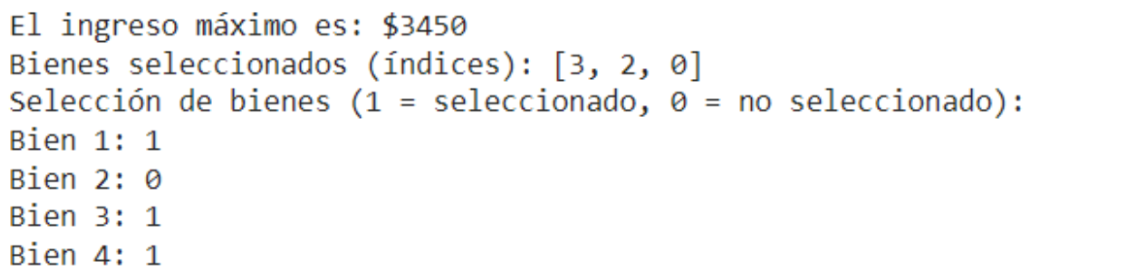
\includegraphics[width=0.8\textwidth]{resultado_mochila_ejem2.png}
    \caption{Imagen del resultado del código Python.}
    \label{fig:resultado_ejemplo2}
\end{figure}

\subsubsection{Análisis de complejidad}
\begin{figure}[H]
    \centering
    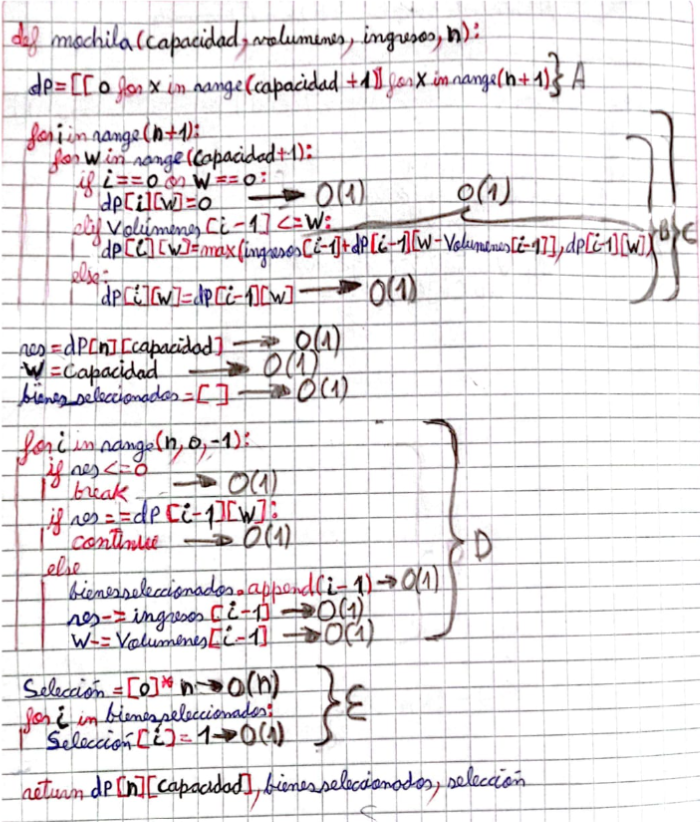
\includegraphics[width=0.8\textwidth]{complejidad_mochila_ejem2.png}
    \caption{Análisis del código.}
    \label{fig:complejidad_ejemplo2}
\end{figure}

\begin{figure}[H]
    \centering
    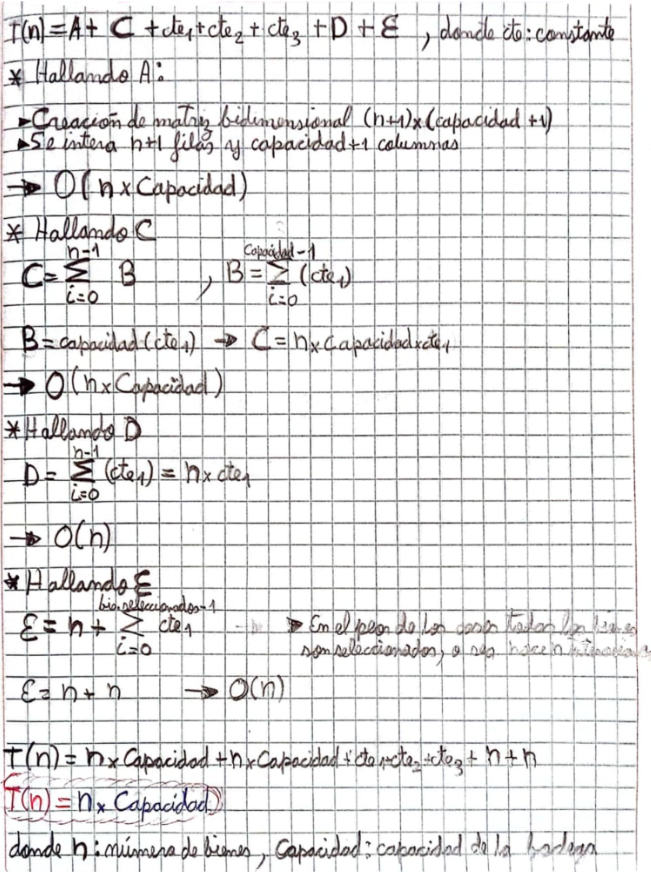
\includegraphics[width=0.8\textwidth]{complejidad_mochila_ejem2_2.png}
    \caption{Análisis del código.}
    \label{fig:complejidad_ejemplo2_2}
\end{figure}

Como se acaba de apreciar, el presente algoritmo tiene una complejidad aproximada de O(n x K) o, equivalentemente, n x capacidad, lo cual supone eficiencia en función al dato de entrada de “capacidad”; mientras más sea esto, más complejo se vuelve.
